% chap2.tex
\part{시뮬레이션 알고리즘}
\label{part:algorithm}

% ---------------------------------------------------------------------------- %
%                                  NEW SECTION                                 %
% ---------------------------------------------------------------------------- %

\chapter{시뮬레이션의 절차 및 구조}

\section{시뮬레이션 절차}
시뮬레이션을 하려면.. 일단 데이터를 읽고 변환하고 옵션 설정해서 돌리고 결과 나온거 정리해서 return함.

% ---------------------------------------------------------------------------- %
%                                  NEW SECTION                                 %
% ---------------------------------------------------------------------------- %

\section{데이터 변환 절차}
json구조로 들어온 데이터는... 동일한 python 구조체로 변환되고.. 그게 dragon이라는 EP친화적 구조체로 변환된 다음 idf로 내보내짐.

% ---------------------------------------------------------------------------- %
%                                  NEW SECTION                                 %
% ---------------------------------------------------------------------------- %

\section{시뮬레이션 조건}
\subsection{기상데이터}
기상데이터는 전국 241개 시군구에서 40?개 지역의 기상데이터로 위도 경도에 따라 mapping된다 (\ref{fig:addr2weather_mapping}). 기상데이터는 국제적으로 통용되는 플랫폼인 climate.onebuilding\cite{onebuilding2024}에서 다운받았다.

\begin{defaultfigure}
  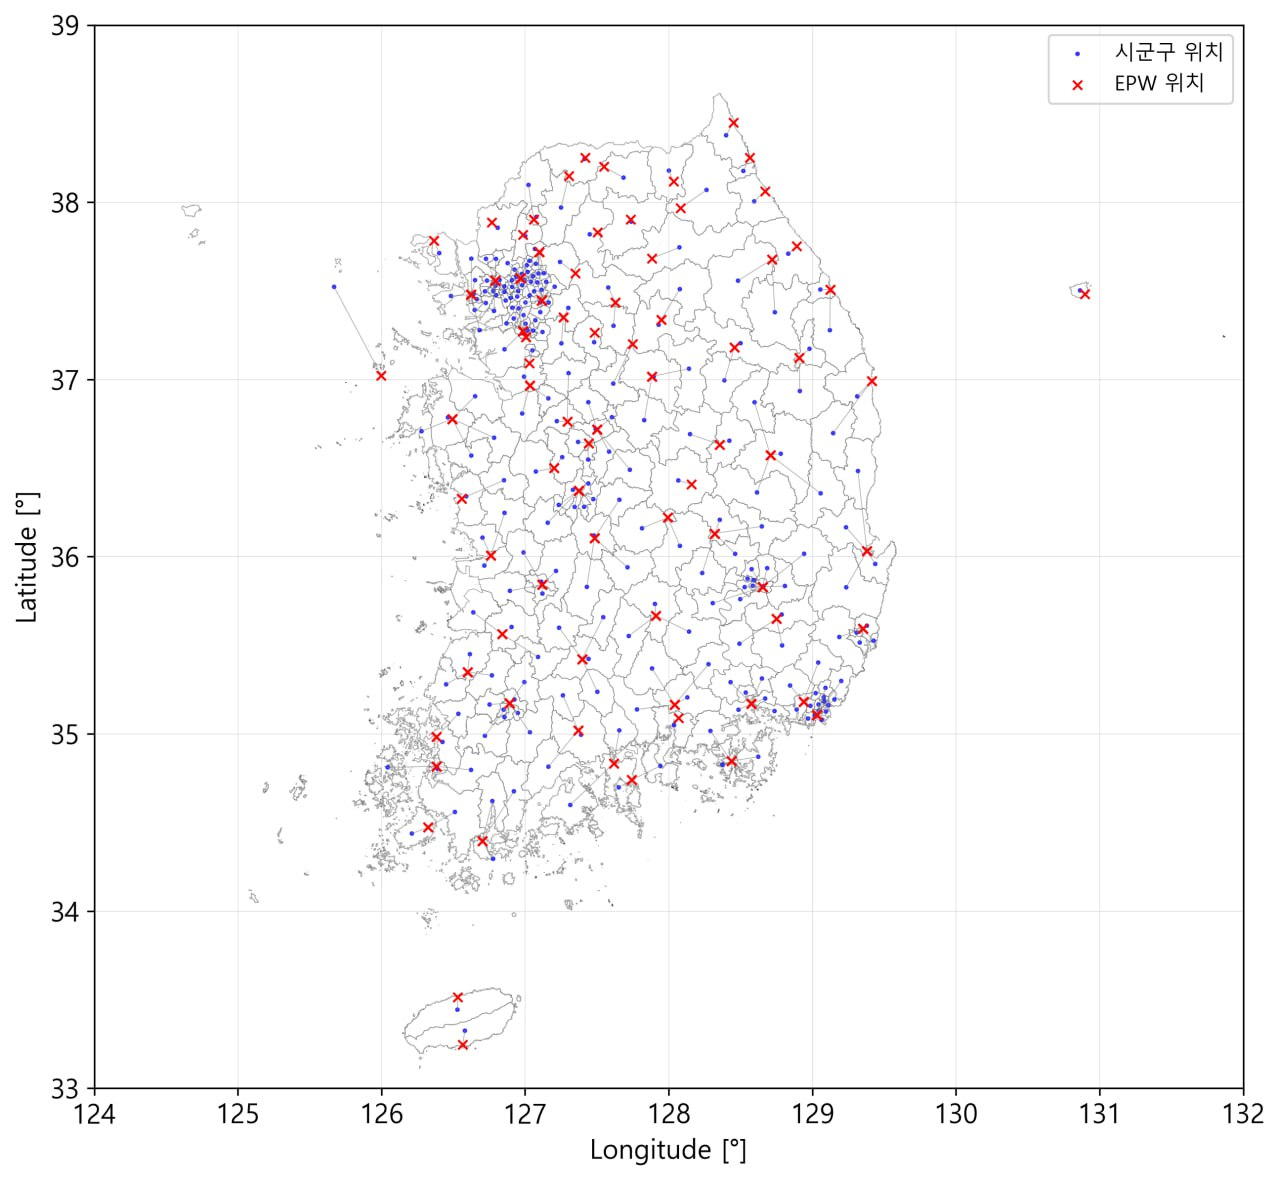
\includegraphics{기상데이터_지역매칭결과.jpg}
  \caption{전국 시군구와 기상데이터 위치}
  \label{fig:addr2weather_mapping}
\end{defaultfigure}


\subsection{EnergyPlus 옵션}
EnergyPlus 레벨에서 정의할 수 있는 시뮬레이션 옵션은 주로, ... , ... 가 있음.
\paragraph{Timestep} 6으로 함. 10분에 한번씩 연산한다는 의미임. EnergyPlus는 4 이상을 권장하고 있음.
\paragraph{DesignCondition} 제일 더운 날, 제일 추운 날을 기상데이터에서 뽑아서 처리함. 일반적인 방식임.

% ---------------------------------------------------------------------------- %
%                                  NEW SECTION                                 %
% ---------------------------------------------------------------------------- %

\section{EnergyPlus 구동}
\subsection{EnergyPlus 실행}
\subsubsection{EnergyPlus의 독립 구동 방법}
EnergyPlus 핵심은 EnergyPlus.exe 맞나? 그것임.
그 전에 expansion 필요하면 expandobject.exe도 실행해주어야 함.
각각은 아래 option들을 받을 수 있음.

\subsection{디렉토리 구조}
코드 내부적으로는 이렇게 호출하고 있는데,
디렉토리는 중간에 3개의 temp 폴더가 생김.
temp 폴더 경로는 C:/users/.../Appdata/Local/Temp/하위에 생김

% ---------------------------------------------------------------------------- %
%                                  NEW SECTION                                 %
% ---------------------------------------------------------------------------- %

\section{오류의 정의와 처리}
오류가 날 수도 있는데, 분류별로 보면 입력이 잘못된 경우와 뭐가 잘못된 경우와... \dots
각각에 대하여는 이렇게 이렇게 처리할 수 있음.
\subsection{입력변수가 잘못된 경우}
입력변수 오류는 python 객체로 전환될 때 탐지해서 이런식으로 return함. 사용자는 이걸 보고 무엇을 판단할 수 있음.
\subsection{idf 변환 과정이 잘못된 경우}
이건 내잘못인데
\subsection{EP가 안돌아가는 경우}
이것도 내잘못임. report하게 만들어뒀으니 실행한 건물이랑 같이 hyeonggon.jo@snu.ac.kr로 제보 바람

% ---------------------------------------------------------------------------- %
%                                  NEW SECTION                                 %
% ---------------------------------------------------------------------------- %

\chapter{항목별 idf 변환 방법}

\section{형상 변환 알고리즘}
\subsection{Simulator 형상 데이터의 구조와 이해}
Simulator는 SG임

\subsection{EnergyPlus 형상 데이터의 구조와 이해}
EnergyPlus는 DG임

\subsection{형상 변환 방법}
좌표 생성하고 뒤집고 copy하고 ...

\subsubsection{좌표 생성}
천장은 높이 받아서 생성하고 나머지도 높이 받아서 만들고 바닥 만들고.
Azimuth는 hash함수로 랜덤하게 생성함. copy한 얘들끼리 180도 뒤집도록 잘 했음

\subsubsection{clone 객체 생성}
이걸 뒤집어서 복제할 것임

\subsubsection{연산 옵션 설정}
그 일사 그림자 계산 옵션은 꺼야함

% ---------------------------------------------------------------------------- %
%                                  NEW SECTION                                 %
% ---------------------------------------------------------------------------- %

\section{구조체 정의}
\subsection{EnergyPlus 구조체의 정의 및 변환 방법}
\subsection{모르는 값 추정}
기축건물은 구조체를 모르는 경우가 많음. 창호는 성적서 없는 경우도 많고... 재료는 어디 써있지도 않음...
\subsubsection{재료}
재료는 여기저기서 소스 모아서 만들어봤음
\begin{defaulttable}
  \caption{기본 재료 물성치}
  \begin{tabularx}{\textwidth}{X X X X X X}
    \toprule
    재료명 (영문,코드) & 재료명(국문) & 열전도도 [$W/m^{2}\cdot K$] & 밀도 [$kg/m^{3}$] & 비열 [$J/kg\cdot K$] & 출처 \\
    \midrule
    concrete   & 콘크리트 & 2.5 & 2400 & 880 & 어디선가 봄\\
    insulation & 단열재   & 0.05 & 30 & 1500 & 봤을지도?  \\
    \bottomrule
  \end{tabularx}
\end{defaulttable}

\subsubsection{구조체}
구조체는 에절서에서 다 긁어모았음. 그냥 콘크리트랑 단열재만 가지고 만듦. 실내외 표면열전달저항도 에절서에서 긁어왔음. RC diagram으로 생각하면 아래 그림과 같은 형태인 것임. 구조체 만들때는 이걸 맞춘거니까 이거 쓰는게 맞음.\par
참고로 EnergyPlus에서는 실내외 표면열전달저항 동적으로 계산됨. 수식은 아래와 같고, 시뮬레이션 해보니 보통 아래와 같음. 비교해보면 차이는 있긴 함.
\begin{tcolorbox}[colback=gray!10, colframe=gray!80, boxrule=0.5pt, left=1em, right=1em]
대충 1년간 hout hin 변화하는 그림 (에절서에 정의된 값이랑 비교할 것) -> 이런 얘기할 때 test건물에 대한 정의는 어떻게 해야 되나? test건물들을 만들어두고 문서 부록에서 기술하여야 할 듯
\end{tcolorbox}

\subsubsection{창호}
창호는 법규에서 U값은 지정하고 있음. SHGC가 없어서 문제임. 또 현장에서 알 수가 없는 경우가 많음. 그래서 그냥 창호 종류에 따라 U, SHGC값을 선택하도록 만들었음.
이것도 에절서 긁었는데, 현재 기준에 있는 걸로 긁었음. 참고로 에절서에 있는 창호 종류별 성능은 에절서 제정된 2013년 이후로 바뀐 적 없음.


% ---------------------------------------------------------------------------- %
%                                  NEW SECTION                                 %
% ---------------------------------------------------------------------------- %

\section{프로필 정의와 활용}
\subsection{ECO2 프로필의 정의}
건기연이 조사해서 이런식으로 정리한 것임. source 값들은 이런게 알려져있음.

\subsection{EnergyPlus 프로필의 정의}
constant도 있고 하지만 simple?그뭐지 그거쓰면 대충 그림 \ref{fig:ep_profile_structure}\와 같이 구별됨

\begin{defaultfigure}
  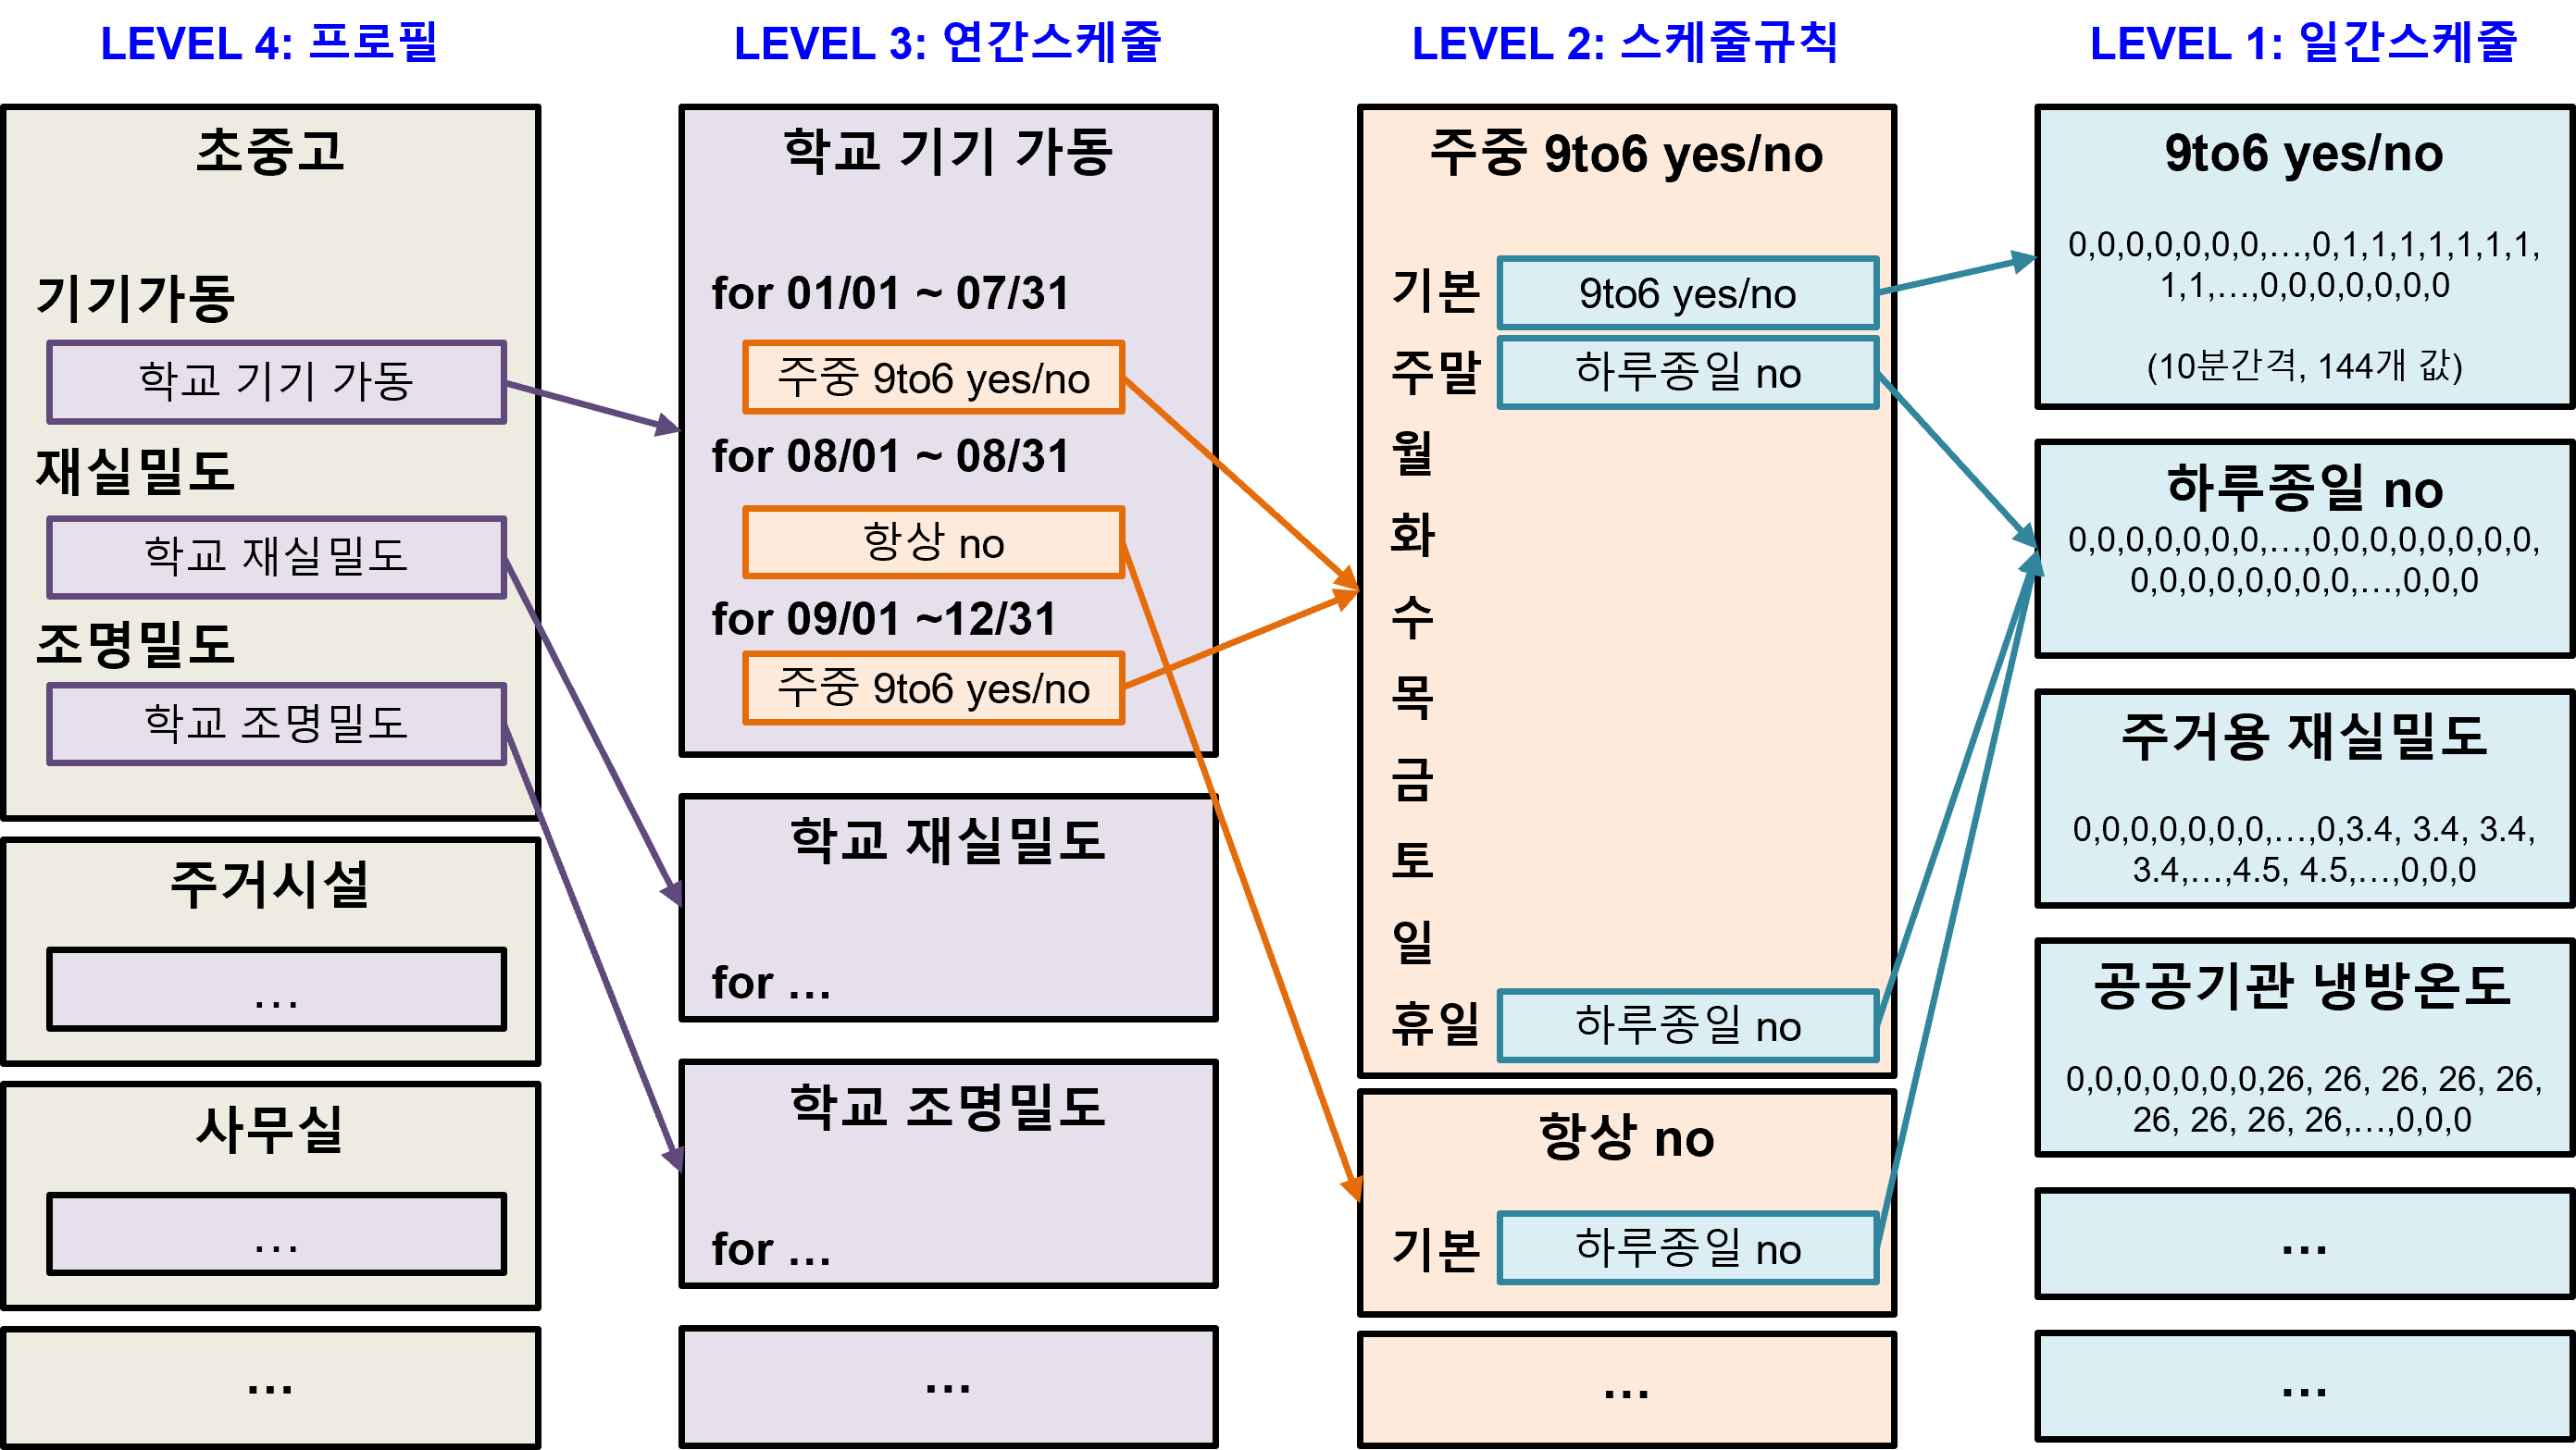
\includegraphics[width=\textwidth]{프로필구조도.png}
  \caption{EP 프로필 구조 예시}
  \label{fig:ep_profile_structure}
\end{defaultfigure}

\subsection{ECO2 프로필을 EnergyPlus 프로필로 변환 방법}
단위는 이렇게 맞추고 나누고 쪼개고 하면 됨

\subsection{신규 프로필 정의 방법}
\subsubsection{직접 정의하는 방법}
직접 한다면 하나하나 정의하면 되겠죠?

\subsubsection{form에 기반하는 방법}
부동산원 과업 대상지는 기본적으로 이런 입력을 지원할 수 있음.
Simulator에 탑재가 될 지는 나도 잘 모르겠네...

% ---------------------------------------------------------------------------- %
%                                  NEW SECTION                                 %
% ---------------------------------------------------------------------------- %

\section{설비 변환 알고리즘}
\subsection{Simulator 설비 데이터의 구조와 이해}
공급-생산 이원화함

\subsection{EnergyPlus 설비 데이터의 구조와 이해}
branch와 loop 개념임

\subsection{설비 변환 방법}
\subsubsection{데이터 구조 변환}
공급 만들고, 생산 만들면 일단 loop만들고 branch 만듦.
그거 결합하면 됨.
필요하면 source의 source도 있음.

\subsubsection{모르는 값 추정}
default 값 쓰는 걸 기본으로 함. 어쨌든 결정해야 했던 것들도 물론 있음.
\paragraph{냉각탑} defulat씀. 그 뭔 기본 팬 제어 채택함
\paragraph{냉동기} defulat씀. 그 뭔 기본 팬 제어 채택함
\paragraph{보일러} defulat씀. 그 뭔 기본 팬 제어 채택함

% ---------------------------------------------------------------------------- %
%                                  NEW SECTION                                 %
% ---------------------------------------------------------------------------- %

\chapter{시뮬레이션 결과의 해석}

\section{EnergyPlus의 실행 결과물 종류와 의미}
table도 나오고 csv도 나오고... 이것저것 다 나옴. 잘 해야 함. 연료별로 table을 생성하고 읽어들임.

\subsection{EP 결과 내는 법과 의미}
Table:Output 어쩌고 활용함. Output은 6가지로 구분되는데, heating, cooling, lighting, fan, pump, cogeneration, ...

\subsubsection{heating}
뭐뭐뭐뭐를 포함함

\subsubsection{cooling}
뭐뭐뭐뭐를 포함함

\subsubsection{lighting}
뭐뭐뭐뭐를 포함함

\subsubsection{fan}
뭐뭐뭐뭐를 포함함.
예를들어, 전열교환기를 설치하는 경우 전열교환기 팬이 사용하는 전력은 여기에 들어감.
nn절에 따라 전열교환기를 모델링하면 전열교환기 1대당 보통 00kW 수준의 전력을 소비함.

\subsubsection{pump}
뭐뭐뭐뭐를 포함함. 예를들어, ...

\subsubsection{cogeneration}
뭐뭐뭐뭐를 포함함

\subsection{EP 결과 읽는 법과 의미}
우리가 원하는 결과는 냉방, 난방, 조명, 유체동력계, 급탕, 발전임.
각각 heating, cooling, lighting, fan과 pump, domestic hot water, cogeneration에 대응됨.

% ---------------------------------------------------------------------------- %
%                                  NEW SECTION                                 %
% ---------------------------------------------------------------------------- %

\section{그린리모델링을 위한 결과 해석}

\subsection{단위면적당 에너지소비량}
보통 그러듯이 EUI 씀. 여기서 단위면적당에는 ....까지 포함임. ECO2랑 다르게 우리는 냉방면적 난방면적 그런거 안함.
바닥면적은 그냥 공조하는 모든 zone의 바닥면적의 총합임.

\subsection{산출 지표들}
월별, 용도별, 원별 에너지사용량이 kWh 단위로 나오면, 국가통계 등에 기반하여 1차에너지소요량, 온실가스 배출량, 비용을 계산할 수 있음.

\subsubsection{1차에너지소요량}\todo{형곤}{형진이 해주삼}\todo{형진}{ㅇㅋ}
열원별 1차에너지환산계수는 아래 표와 같음. 이거는 명확함\todo{철홍}{명확하지 않은 듯}. 매년 x월 업데이트 되고 있으므로 본 시뮬레이터도 업데이트 필요함.

\subsubsection{온실가스 배출량}\todo{승주}{이건 두번째 레슨}
온실가스는 CO2eq로 계산하는게 표준임. eq 계산은 어떻게 함. 온실가스 종류별 CO2변환계수(지구온난화지수?)는 아래 표 참고 바람. \par
\todo{아무거나}{광역어그로}
\todo{무거나아}{전역어그로}
전기는 어떻게 계산함. \par
가스는 어떻게 계산함. \par
등유는 어떻게 계산함. 이건 좀 복잡한데, IPCC에서... 이런 수식을 사용하고 있고, 이런 표를 제시하고 있고, 그 값은 아래 표와 같고... \par
지역난방은 어떻게 계산함. 이건 더 복잡한데...\par

계산한 값은 아래 표와 같음. 

\subsubsection{비용}
비용은 워낙 체계가 복잡해서 퉁치는 접근을 취함. 이거 똑바로 계산하라그러면 쉽지 않음.
전기는 어떻게 계산함. \par
가스는 어떻게 계산함. \par
등유는 어떻게 계산함. 이건 좀 복잡한데, IPCC에서... 이런 수식을 사용하고 있고, 이런 표를 제시하고 있고, 그 값은 아래 표와 같고... \par
지역난방은 어떻게 계산함. 이건 더 복잡한데...\par

계산한 값은 아래 표와 같음. 


